%==========================================================
\section{Exercise 1}\label{sec:ex1}
%==========================================================
In Figure \ref{fig:ex1} I show that 
\begin{align*}
    \quad \frac{\partial (\mathbf{a}^{T}\mathbf{x})}{\partial \mathbf{x}} &= \mathbf{a}^{T} && \text{and} & \frac{\partial (\mathbf{a}^{T} \mathbf{A} \mathbf{a})}{\partial \mathbf{a}} &= \mathbf{a}^{T} (\mathbf{A} \mathbf{A}^{T}) && \text{and} & \frac{\partial (\mathbf{x} - \mathbf{A} \mathbf{s})^{T} (\mathbf{x} - \mathbf{A} \mathbf{s})}{\partial \mathbf{s}} &= -2 (\mathbf{x} - \mathbf{A} \mathbf{s})^{T} \mathbf{A}
\end{align*}

\begin{figure}
    \centering
    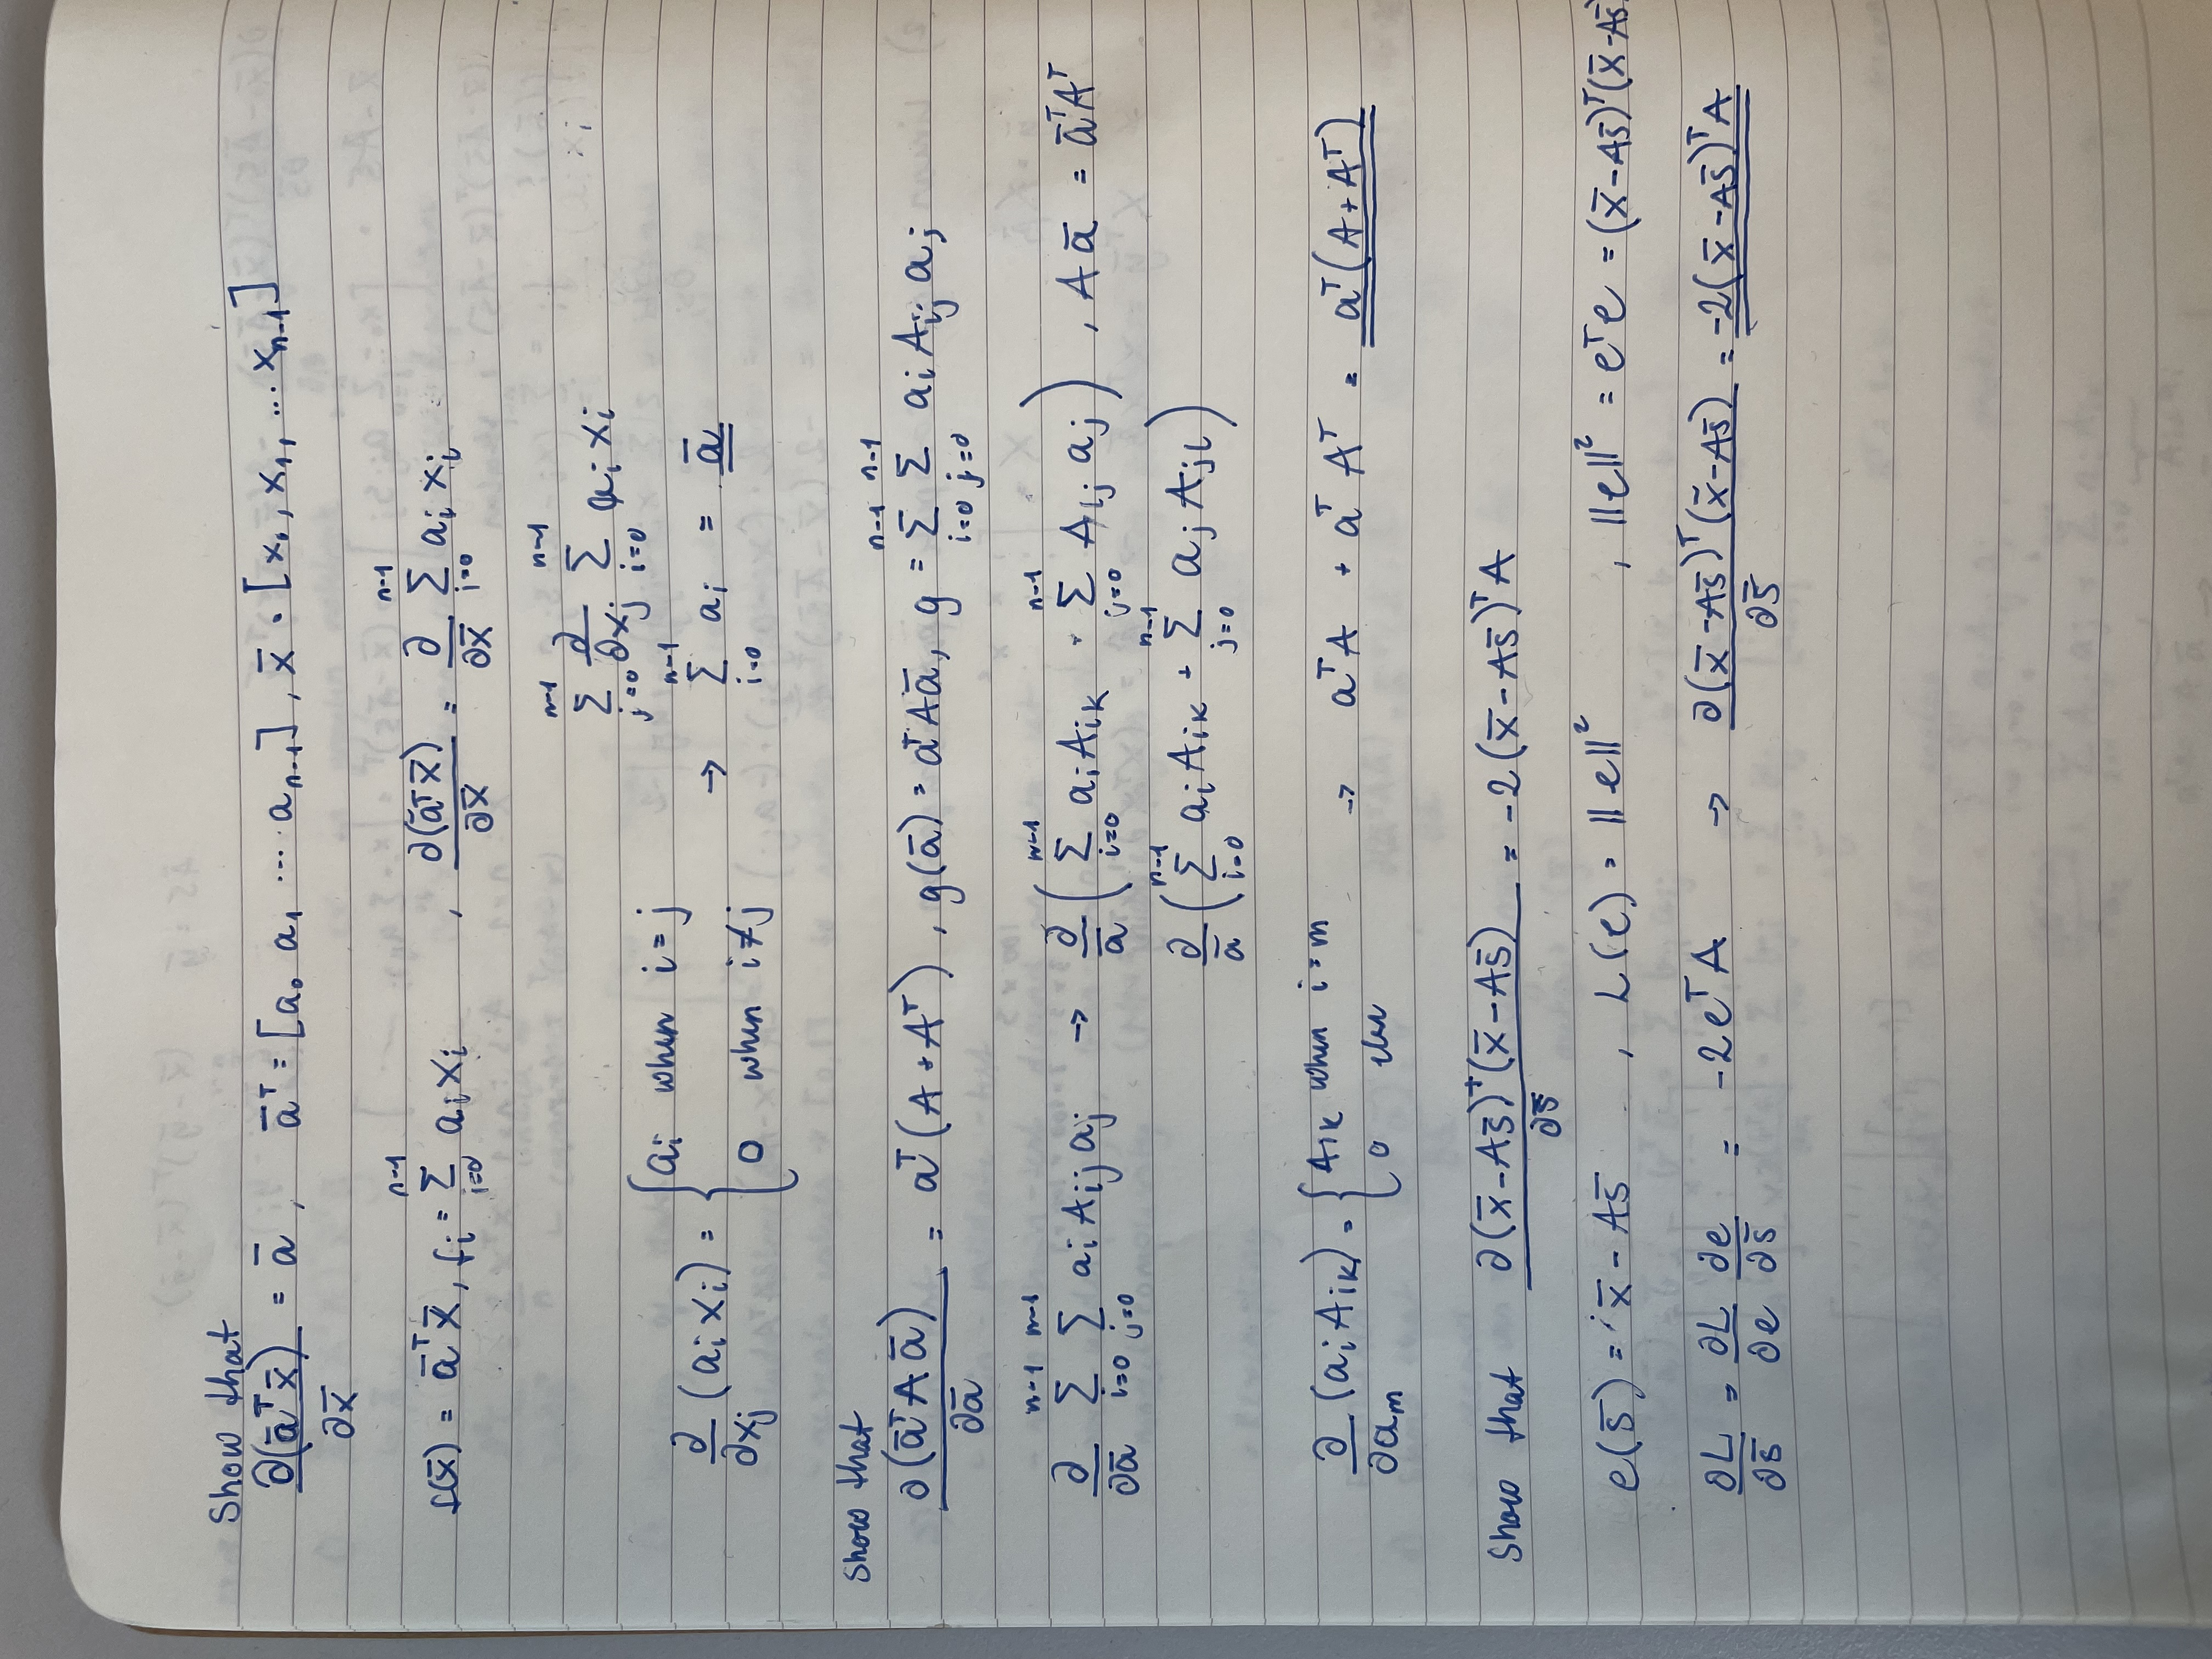
\includegraphics[width=0.8\linewidth, angle=270]{latex/figures/ex35-1.jpeg}
    \caption{Answer for exercise 1}
    \label{fig:ex1}
\end{figure}

\section{Exercise 2}\label{sec:ex2}
\begin{lstlisting}[language=Python]
import numpy as np
import matplotlib.pyplot as plt
from sklearn.linear_model import LinearRegression
from sklearn.preprocessing import PolynomialFeatures
from sklearn.metrics import mean_squared_error, r2_score

def exercise_35_2():
    x = np.random.rand(100)
    y = 2.0 + 5*x**2 + 0.1*np.random.randn(100)

    # Create design matrix 
    X = np.zeros((len(x), 3))
    X[:, 0] = 1
    X[:, 1] = x 
    X[:, 2] = x*x 

    beta = np.linalg.inv(X.T @ X) @ X.T @ y 
    y_pred = X @ beta

    poly = PolynomialFeatures(degree=2)
    X_model = poly.fit_transform(x[:, np.newaxis])
    model = LinearRegression()
    model.fit(X, y)
    model_pred = model.predict(X_model)

    mse_man = mean_squared_error(y, y_pred)
    r2_man = r2_score(y, y_pred)
    mse_sk = mean_squared_error(y, model_pred)
    r2_sk = r2_score(y, model_pred)
    
    fig, ax = plt.subplots()
    ax.plot(x, y, 'b.', label="Data")
    ax.plot(x, y_pred, 'ro', label=f"Own code: MSE = {mse_man:.4f}, R2 = {r2_man:.4f}")
    ax.plot(x, model_pred, 'gx', label=f"SciKit: MSE = {mse_sk:.4f}, R2 = {r2_sk:.4f}")
    ax.legend()
    plt.show()
\end{lstlisting}

\begin{figure}
    \centering
    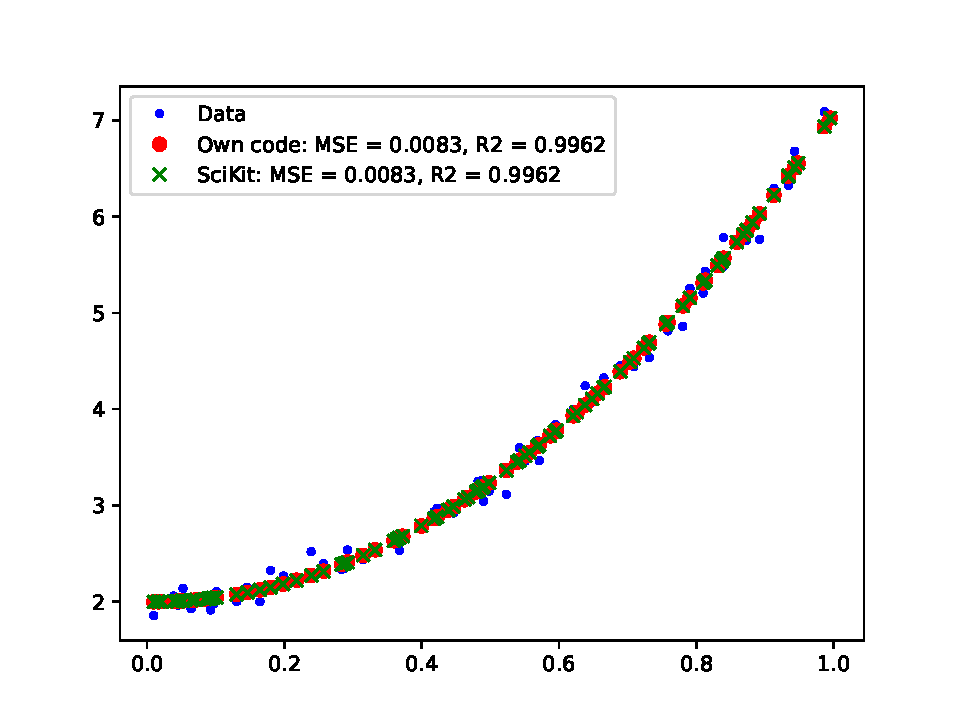
\includegraphics[width=0.5\linewidth]{latex/figures/week35_ex2.pdf}
    \caption{Results for exercise 2}
    \label{fig:ex2}
\end{figure}

\section{Exercise 3}\label{sec:ex3}
\begin{lstlisting}[language=Python]
class LinRegression:

    def __init__(self, degree) -> None:
        self._degree = degree + 1

    def _design_matrix(self, x):
        X = np.zeros((len(x), self._degree))
        X[:, 0] = 1
        for i in range(1, self._degree):
            X[:, i] = x**i
        return X

    def fit(self, x_train, y_train):
        self._X = self._design_matrix(x_train)
        self._X_T = self._X.T
        self._beta = np.linalg.inv(self._X_T @ self._X) @ self._X_T @ y_train 

    def predict(self, x_test):
        X_test = self._design_matrix(x_test)
        y_pred = X_test @ self._beta
        return y_pred 
    
    def compute_error(self, y_true, y_pred):
        self._mse = mse(y_true, y_pred)
        self._r2 = r2(y_true, y_pred)
        return self._mse, self._r2
        
def exercise_35_3():
    n = 100
    
    x = np.linspace(-3, 3, n)
    # x = x.reshape(-1, 1)
    noise = np.random.normal(0, 0.1, x.shape)
    y = np.exp(-x**2) + 1.5 * np.exp(-(x-2)**2) + noise 

    # poly = PolynomialFeatures(degree=4)
    # X = poly.fit_transform(x[:, np.newaxis])

    x_train, x_test, y_train, y_test = train_test_split(x, y, test_size=0.2)

    mse_history = []
    r2_history = []

    for degree in range(15):
        model = LinRegression(degree)
        model.fit(x_train, y_train)
        y_pred = model.predict(x_test)
        mse_loss, r2_val = model.compute_error(y_test, y_pred)
        mse_history.append(mse_loss)
        r2_history.append(r2_val)

    d = np.arange(15)
    fig, ax = plt.subplots()
    ax.plot(d, mse_history, label="MSE")
    ax.plot(d, r2_history, label="R2")
    ax.legend()
    plt.show()
    print(f"Optimal MSE = {mse_history[8]:.4f}, polynomial degree = {np.argmin(mse_history)}")
\end{lstlisting}

\begin{figure}
    \centering
    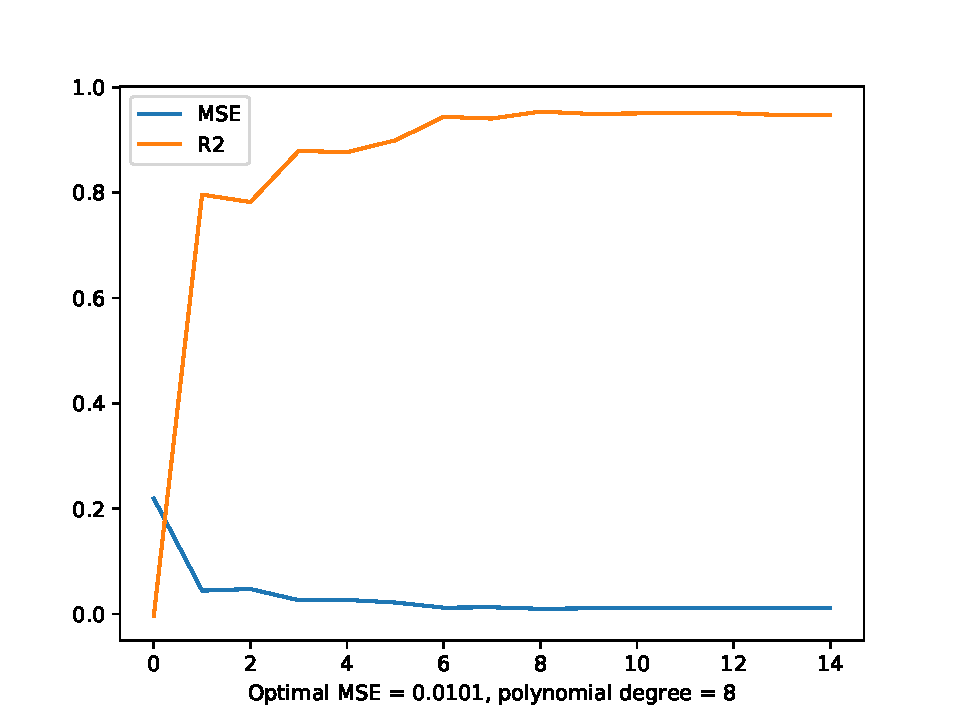
\includegraphics[width=0.5\linewidth]{latex/figures/week35_ex3.pdf}
    \caption{Results for exercise 3}
    \label{fig:ex3}
\end{figure}